\documentclass[twoside,a4paper,11pt]{article}
\usepackage[preprint]{irrj2e}
\usepackage[T1]{fontenc}
\usepackage{amsmath,booktabs,pgfplots,array,longtable,xurl}
\emergencystretch=1em
\setcounter{topnumber}{4}\setcounter{totalnumber}{5}
\renewcommand{\topfraction}{.95}\renewcommand{\textfraction}{.05}\renewcommand{\floatpagefraction}{.8}
\pgfplotsset{compat=1.18}
\ShortHeadings{Evidence Sets and Retrieval Evaluation}{Lin}
\firstpageno{1}
\begin{document}
\title{Supplementary material: When Evidence Sets Become Relevance Lists: A Controlled Audit of Scientific Retrieval Evaluation}
\author{\name Yunya Lin \\ \addr University of Illinois Urbana-Champaign}
\maketitle
\begin{abstract}Supplementary distributions, implementation-audit details, encoder feasibility evidence, and computational provenance for the controlled evaluation study. No additional effectiveness experiment is reported.\end{abstract}
\begin{keywords}retrieval evaluation; evidence sets; scientific information; measurement validity; reproducibility\end{keywords}

\section{Additional depth distributions and tabulated results}
Figure 1 shows the cumulative distribution of additional ranked depth. Its zero mass is central to interpretation: the BM25 median is zero in each corpus despite positive mean cost. The scientific results and definitions are the same as in the main article.

\begin{figure}[!htbp]\centering
\hbox to\textwidth{\begin{minipage}{.48\textwidth}\centering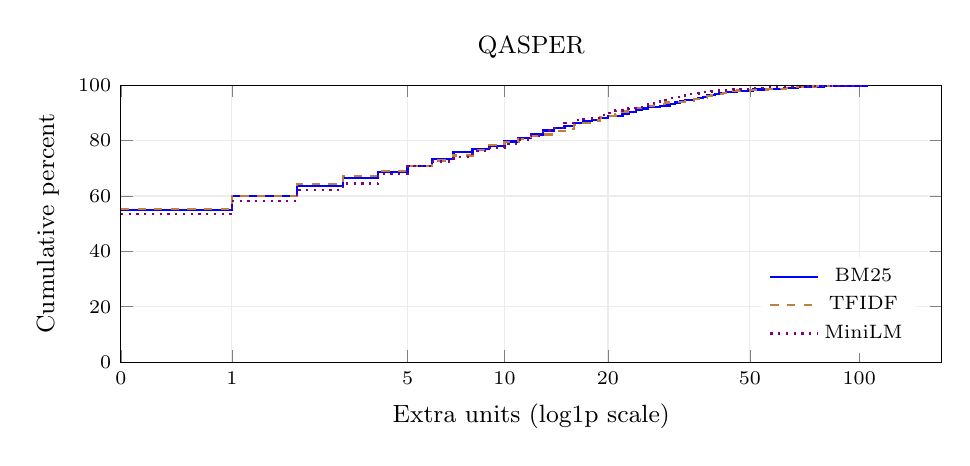
\begin{tikzpicture}\begin{axis}[width=.99\linewidth,height=5.1cm,tick label style={font=\scriptsize},label style={font=\small},title style={font=\small},title=QASPER,grid=major,grid style={gray!15},legend style={font=\scriptsize,draw=none},legend pos=south east,xmin=0,ymin=0,ymax=100,xlabel={Extra units (log1p scale)},ylabel={Cumulative percent},xtick={0,.693147,1.791759,2.397895,3.044522,3.931826,4.615121},xticklabels={0,1,5,10,20,50,100}]
\addplot[const plot,thick,blue,solid] coordinates {(0.00000000,54.85714286) (0.69314718,60.00000000) (1.09861229,63.54285714) (1.38629436,66.40000000) (1.60943791,68.68571429) (1.79175947,70.74285714) (1.94591015,73.37142857) (2.07944154,75.88571429) (2.19722458,77.02857143) (2.30258509,78.05714286) (2.39789527,79.65714286) (2.48490665,80.80000000) (2.56494936,82.17142857) (2.63905733,83.65714286) (2.70805020,84.45714286) (2.77258872,85.37142857) (2.83321334,86.28571429) (2.89037176,87.08571429) (2.94443898,87.42857143) (2.99573227,88.22857143) (3.04452244,88.91428571) (3.13549422,89.60000000) (3.17805383,90.40000000) (3.21887582,90.97142857) (3.25809654,91.54285714) (3.29583687,92.11428571) (3.33220451,92.22857143) (3.36729583,92.45714286) (3.40119738,92.68571429) (3.43398720,93.25714286) (3.46573590,93.71428571) (3.49650756,94.05714286) (3.52636052,94.51428571) (3.55534806,94.74285714) (3.58351894,94.85714286) (3.61091791,95.31428571) (3.63758616,95.77142857) (3.66356165,96.22857143) (3.68887945,96.57142857) (3.71357207,96.91428571) (3.73766962,97.02857143) (3.76120012,97.14285714) (3.78418963,97.60000000) (3.82864140,97.71428571) (3.85014760,97.82857143) (3.91202301,97.94285714) (3.93182563,98.05714286) (3.95124372,98.40000000) (4.02535169,98.51428571) (4.04305127,98.62857143) (4.06044301,98.74285714) (4.14313473,99.08571429) (4.23410650,99.20000000) (4.24849524,99.31428571) (4.27666612,99.42857143) (4.31748811,99.54285714) (4.39444915,99.65714286) (4.40671925,99.77142857) (4.46590812,99.88571429) (4.66343909,100.00000000)};
\addlegendentry{BM25}
\addplot[const plot,thick,brown,dashed] coordinates {(0.00000000,55.20000000) (0.69314718,60.00000000) (1.09861229,64.22857143) (1.38629436,67.08571429) (1.60943791,69.02857143) (1.79175947,70.85714286) (1.94591015,72.80000000) (2.07944154,74.62857143) (2.19722458,76.57142857) (2.30258509,78.28571429) (2.39789527,79.54285714) (2.48490665,80.57142857) (2.56494936,81.60000000) (2.63905733,82.17142857) (2.70805020,83.31428571) (2.77258872,84.11428571) (2.83321334,85.60000000) (2.89037176,86.28571429) (2.94443898,87.20000000) (2.99573227,88.34285714) (3.04452244,88.80000000) (3.09104245,89.37142857) (3.13549422,90.51428571) (3.17805383,91.65714286) (3.21887582,91.88571429) (3.25809654,92.22857143) (3.29583687,92.34285714) (3.33220451,93.02857143) (3.36729583,93.14285714) (3.40119738,93.71428571) (3.43398720,93.82857143) (3.49650756,93.94285714) (3.52636052,94.05714286) (3.55534806,94.40000000) (3.58351894,94.97142857) (3.61091791,95.42857143) (3.63758616,95.54285714) (3.66356165,96.00000000) (3.68887945,96.22857143) (3.71357207,96.34285714) (3.73766962,96.68571429) (3.76120012,97.14285714) (3.78418963,97.48571429) (3.80666249,97.71428571) (3.82864140,97.94285714) (3.85014760,98.05714286) (3.93182563,98.17142857) (3.97029191,98.28571429) (4.00733319,98.40000000) (4.04305127,98.51428571) (4.07753744,98.62857143) (4.12713439,98.74285714) (4.15888308,99.08571429) (4.18965474,99.20000000) (4.20469262,99.31428571) (4.23410650,99.42857143) (4.29045944,99.54285714) (4.34380542,99.65714286) (4.35670883,99.77142857) (4.36944785,99.88571429) (4.44265126,100.00000000)};
\addlegendentry{TFIDF}
\addplot[const plot,thick,violet,dotted] coordinates {(0.00000000,53.37142857) (0.69314718,58.05714286) (1.09861229,62.05714286) (1.38629436,64.45714286) (1.60943791,68.00000000) (1.79175947,70.85714286) (1.94591015,72.45714286) (2.07944154,73.94285714) (2.19722458,76.11428571) (2.30258509,77.37142857) (2.39789527,78.85714286) (2.48490665,80.34285714) (2.56494936,81.82857143) (2.63905733,83.65714286) (2.70805020,84.45714286) (2.77258872,86.28571429) (2.83321334,87.31428571) (2.89037176,87.88571429) (2.94443898,88.22857143) (2.99573227,89.14285714) (3.04452244,89.94285714) (3.09104245,90.85714286) (3.13549422,91.54285714) (3.17805383,91.77142857) (3.21887582,92.11428571) (3.25809654,92.91428571) (3.29583687,93.14285714) (3.33220451,93.94285714) (3.36729583,94.28571429) (3.40119738,94.74285714) (3.43398720,95.31428571) (3.46573590,95.65714286) (3.49650756,96.11428571) (3.52636052,96.45714286) (3.55534806,96.91428571) (3.61091791,97.60000000) (3.68887945,97.71428571) (3.71357207,97.94285714) (3.73766962,98.05714286) (3.78418963,98.17142857) (3.80666249,98.28571429) (3.82864140,98.40000000) (3.87120101,98.51428571) (3.89182030,98.62857143) (3.91202301,98.74285714) (3.95124372,98.85714286) (3.98898405,98.97142857) (4.00733319,99.08571429) (4.02535169,99.20000000) (4.04305127,99.31428571) (4.07753744,99.42857143) (4.27666612,99.54285714) (4.30406509,99.65714286) (4.49980967,99.77142857) (4.54329478,99.88571429) (4.63472899,100.00000000)};
\addlegendentry{MiniLM}\end{axis}\end{tikzpicture}\end{minipage}\hfill\begin{minipage}{.48\textwidth}\centering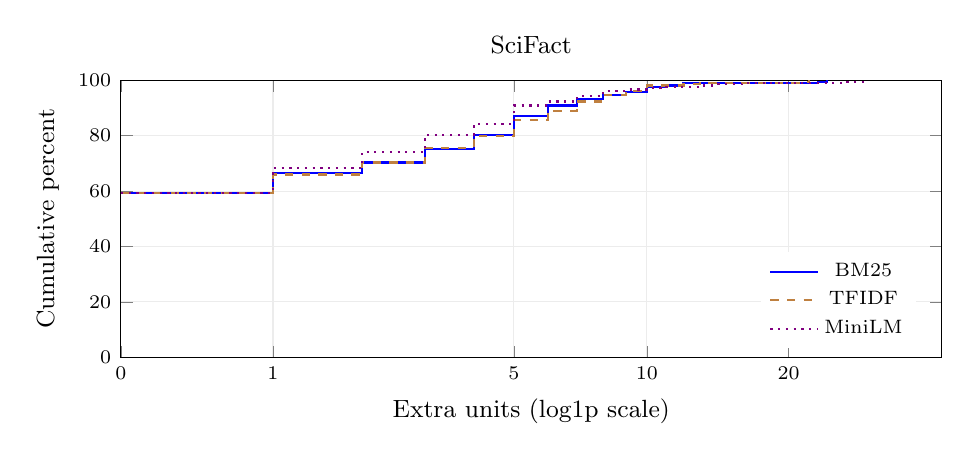
\begin{tikzpicture}\begin{axis}[width=.99\linewidth,height=5.1cm,tick label style={font=\scriptsize},label style={font=\small},title style={font=\small},title=SciFact,grid=major,grid style={gray!15},legend style={font=\scriptsize,draw=none},legend pos=south east,xmin=0,ymin=0,ymax=100,xlabel={Extra units (log1p scale)},ylabel={Cumulative percent},xtick={0,.693147,1.791759,2.397895,3.044522,3.931826,4.615121},xticklabels={0,1,5,10,20,50,100}]
\addplot[const plot,thick,blue,solid] coordinates {(0.00000000,59.33014354) (0.69314718,66.50717703) (1.09861229,70.33492823) (1.38629436,75.11961722) (1.60943791,80.38277512) (1.79175947,87.08133971) (1.94591015,90.90909091) (2.07944154,93.30143541) (2.19722458,94.73684211) (2.30258509,95.69377990) (2.39789527,97.60765550) (2.48490665,98.08612440) (2.56494936,99.04306220) (3.17805383,99.52153110) (3.21887582,100.00000000)};
\addlegendentry{BM25}
\addplot[const plot,thick,brown,dashed] coordinates {(0.00000000,59.33014354) (0.69314718,66.02870813) (1.09861229,70.33492823) (1.38629436,75.59808612) (1.60943791,79.90430622) (1.79175947,85.64593301) (1.94591015,88.99521531) (2.07944154,92.34449761) (2.19722458,94.73684211) (2.30258509,96.17224880) (2.39789527,98.08612440) (2.56494936,98.56459330) (2.63905733,99.04306220) (3.09104245,99.52153110) (3.13549422,100.00000000)};
\addlegendentry{TFIDF}
\addplot[const plot,thick,violet,dotted] coordinates {(0.00000000,59.33014354) (0.69314718,68.42105263) (1.09861229,74.16267943) (1.38629436,80.38277512) (1.60943791,84.21052632) (1.79175947,90.90909091) (1.94591015,92.34449761) (2.07944154,94.25837321) (2.19722458,96.17224880) (2.30258509,96.65071770) (2.39789527,97.12918660) (2.48490665,97.60765550) (2.63905733,98.08612440) (2.70805020,98.56459330) (2.83321334,99.04306220) (3.29583687,99.52153110) (3.40119738,100.00000000)};
\addlegendentry{MiniLM}\end{axis}\end{tikzpicture}\end{minipage}}
\caption{Empirical cumulative distributions of extra ranked units for union completion. Horizontal axes are transformed by log(1+extra units), with corpus-specific ranges. The large mass at zero and the tail must be considered together.}
\end{figure}
Machine-readable tables retain all methods and budgets, paired contrasts, original and joint sensitivities, the four disjoint topology categories, singleton/answer-agreement modifiers, and contributions to score and cost. Empty strata remain empty, and cells with fewer than ten represented clusters are flagged sparse. The joint restriction, topology decomposition, implementation audit, and modern-encoder feasibility analysis are post-main and exploratory.


\section{Implementation-audit protocol and evidence}
The implementation audit was frozen before inspecting additional code behavior. Prior familiarity with both official evaluators was disclosed, and those evaluators are reference cases outside downstream counts. On 3 October 2026 UTC, each benchmark name was crossed with ``dataset loader,'' ``evidence retrieval evaluation,'' ``qrels conversion,'' and ``RAG benchmark'' in domain-restricted searches of GitHub and Hugging Face datasets. The first ten available results per query were logged, including exclusions and inaccessible results.

The search comprised sixteen phrase-quoted queries and sixteen benchmark-quoted queries added by a pre-classification amendment, totaling 320 result slots and 148 canonical projects. Three inaccessible QASPER distributions had unverified eligibility. The final eligible pool contained 24 QASPER and 32 SciFact downstream families; fifteen per benchmark were selected by ascending SHA-256 of canonical identifiers. Post-inspection corrections merged the VikingRAG/OpenViking lineage and treated official AllenAI distributions as reference cases, replacing their selected slots with the next eligible families. The protocol, query records, eligibility decisions, and selection correction records accompany the package.

Classification traces pinned input, conversion, output, and scoring roles where accessible. Grouped lists preserve relationships even without explicit set IDs. The classification ledger records commit/revision, code locations, source/output granularity, transformation, supporting evidence, and uncertainty. A second consistency pass rechecked these source records. It does not constitute independent human annotation. Six isolated conversion fixtures supplement static code and schema inspection; no complete downstream model pipeline was executed.

The official QASPER evaluator selects a best reference for Evidence F1. The official SciFact evaluator retains alternative rationales for its complete-rationale abstract-level condition; sentence-level coverage is distinct. The official SciFact Hugging Face loader expands a rationale into a row, permitting grouping by claim and document. Reference distributions are excluded from downstream counts.

For mteb/QASPER, comparison with source IDs finds exact raw-union targets for 576 of 1,335 matched questions. This prevents interpreting every released target as the controlled union intervention. The sscc-rag-paper fixture demonstrates relation loss when every evidence unit maps; real input can additionally lose unmatched evidence. These two failure modes are recorded separately.

Final downstream counts in preserved/flat-only/both/other/undetermined order are QASPER 0/2/3/9/1 and SciFact 1/0/1/13/0. Unavailable and changed-task cases remain visible. These bounded counts do not estimate ecosystem prevalence.


\subsection{Case-selection record}
The frozen error taxonomy contains 306/123/156/290 QASPER items and 34/9/58/108 SciFact pairs in the no-hit, fragment-only, one-set-without-union, and union-complete categories. Earlier examples were selected by SHA-256 order within each category, up to three per category. The panels in the main article present the first already-selected one-set-without-union case from each corpus; they are illustrations, not representative-sample estimates.


\section{Result-blind modern-encoder feasibility gate}
Qwen3-Embedding-0.6B was the sole post-main candidate \citep{qwen}. Its official revision, tokenizer, weights, and separate dependencies were pinned. The proposed configuration used float32 CPU inference, last-token pooling, normalized 1,024-dimensional vectors, an 8,192-token limit, and the fixed instruction ``Given a scientific question or claim, retrieve passages that provide evidence relevant to it.'' Queries were instructed and candidate units were not.

The frozen gate sampled 32 inputs by SHA-256 from each equal-count tokenizer-length quartile, adding its longest input when absent. Timing 132 of 20,112 unique inputs projected 10,568.9 seconds (2.94 hours), exceeding the prespecified two-hour limit. Full inference was therefore omitted. No effectiveness outcomes were computed from the timing sample, and no substitute was tried. The conservative longest-input addition and local runtime conditions limit the precision of this projection; omission leaves the modern-retriever robustness question unresolved.

The pinned Qwen model revision is 97b0c614be4d77ee51c0cef4e5f07c00f9eb65b3. The separate environment records PyTorch 2.8.0 and Transformers 4.57.1, with exact resolved dependencies, tokenizer and weight hashes. Timing and truncation records are separate from the MiniLM embedding cache. The complete projection reconstructs from the length-bin means, full input counts, model loading, and warm-up costs. The gate was applied before effectiveness evaluation.


\section{Answer-agreement implementation}
The frozen function answer\_key in src/evidence.py selects nonempty extractive\_spans first (in source order, joined by comma-space), then nonempty free\_form\_answer, then yes\_no when non-null, and otherwise the empty string. It applies Python str.lower, deletes string.punctuation (ASCII punctuation), removes whole-word a/an/the with a regular expression, and joins whitespace-separated tokens with one space. It does not apply Unicode normalization or delete non-ASCII punctuation. qasper\_instances retains agreement when the set of normalized strings across all annotations has size one. The joint sensitivity in src/supplemental.py uses that saved indicator before minimal-reference pruning.


\section{Computational provenance and replay}
The pilot used SHA-256-selected QASPER development papers and SciFact training claims, yielding 88 and 47 eligible items; none entered the main estimates. Inclusion rules, metrics, models, and analysis were frozen locally at 2026-10-03T00:51:19 UTC. This is a prospective local record, not public preregistration.

QASPER test annotations were first deserialized after the freeze. SciFact development schema and availability had been inspected earlier, but rankings had not been scored. No retriever was tuned on either main cohort. The saved experiment contains 5420 full rankings and 32520 unit-budget scoring points.

The main CPU run took 626.5 seconds on ARM64 macOS with Python 3.12. Input, code, configuration, and model fingerprints bind checkpointed rankings and embedding caches. The reproduction package retains timestamped source snapshots, acquisition hashes, pilot records, correction logs, and current presentation sources.

The MiniLM revision is 1110a243fdf4706b3f48f1d95db1a4f5529b4d41. The acquired SciFact archive is distributed through a mutable latest URL, so acquisition hashes, rather than the URL label, identify this study's annotations. Data and model acquisition manifests and the frozen configuration identify the exact source artifacts.

Adapters validate nonempty evidence families and source-unit mappings. Scores treat predicted IDs as sets; duplicate references do not change H, C, A, or max-reference overlap. Fingerprints bind rankings to queries, units, annotations, configuration, and retrieval code.

The reproduction guide distinguishes replay of saved outputs from new retrieval. Frozen primary outputs and post-main exploratory additions are stored separately, with source fingerprints and machine-readable validation records. External datasets and model weights are acquired from their distributors using the supplied URLs and hashes. The public repository is \url{https://github.com/YoyoLin008/evidence-sets-retrieval-evaluation}.


\section{Literature-search scope}
A final targeted search on 3 October 2026 UTC covered evidence ranking, evidence-set completion, sufficient evidence sets, minimal sufficient rank, multiple gold evidence sets, alternative evidence sets, conjunctive evidence, grouped qrels, structured relevance judgments, flattened qrels, evidence aggregation, and best-reference versus union evaluation. Primary-source records and exact queries are retained in the literature ledger. This is targeted positioning, not a systematic review.

Alt et al. (2026) and Li et al. (2025) were read in full for the comparison of sufficient-set ranking and group-versus-union evaluation \citep{alt2026,li2025}. The claim-to-source ledger distinguishes bibliographic verification from methodological reading and records source-access limitations. Cha et al. and Nguy are cited as preprints.


\section{Authorship and assistance}
Generative AI tools (OpenAI Codex) supported grammar checking, language refinement, clarity, and organization. The author conceived the study, made the substantive methodological and interpretive decisions, conducted and verified the research, and wrote the substantive content. Under the author's direction, tool assistance also supported code edits, reruns, numerical and reference checks, and preparation of figures and manuscript files. The author reviewed AI-assisted material and takes responsibility for the final work. AI is not an author.


\section{Acknowledgments and disclosure of funding}
No external funding or third-party computational resources were received or used for this work. All computational experiments were conducted locally on the author's personal computer.

\clearpage\begin{thebibliography}{99}
\bibitem[Alt et~al.(2026)]{alt2026}
Guy Alt, Eran Hirsch, Serwar Basch, Ido Dagan, Oren Glickman. (2026). User-Centric Evidence Ranking for Attribution and Fact Verification. Proceedings of the 19th Conference of the European Chapter of the Association for Computational Linguistics (Volume 1: Long Papers), pp. 7215--7237. \url{https://aclanthology.org/2026.eacl-long.340/}.

\bibitem[Li et~al.(2025)]{li2025}
Xiangci Li, Sihao Chen, Rajvi Kapadia, Jessica Ouyang, Fan Zhang. (2025). Minimal Evidence Group Identification for Claim Verification. Proceedings of the 5th Workshop on Trustworthy NLP (TrustNLP 2025), pp. 103--111. \url{https://aclanthology.org/2025.trustnlp-main.8/}.

\bibitem[Qwen Team(2025)]{qwen}
Qwen Team. (2025). Qwen3-Embedding-0.6B: Model Card. Hugging Face model documentation, revision 97b0c614be4d77ee51c0cef4e5f07c00f9eb65b3. \url{https://huggingface.co/Qwen/Qwen3-Embedding-0.6B/tree/97b0c614be4d77ee51c0cef4e5f07c00f9eb65b3}.

\end{thebibliography}\end{document}
